% !TEX root = ../Report.tex
% ======================================================================
\chapter{System Design}
\label{ch:design}
% ======================================================================

This chapter describes GiTrip's architecture, data model, and major subsystems:
repository semantics, planner, routing, merging, UI interaction surfaces, and
supporting features. Each section explains not only what was built but why that
approach was chosen over alternatives.

\section{High-level Architecture}
GiTrip is a server-rendered web application with the following architecture:
\begin{itemize}
  \item \textbf{Backend:} Node.js with Express, providing both UI routes (EJS templates) and JSON API endpoints for asynchronous operations.
  \item \textbf{Persistence:} SQLite storing repositories, branches, commits, users (optional), sessions, and collaborators.
  \item \textbf{Frontend:} EJS templates enhanced with client-side JavaScript for map and timeline interactions.
  \item \textbf{Mapping:} Leaflet with OpenStreetMap tiles.
\end{itemize}

As illustrated in Figure~\ref{fig:architecture}, UI routes under \texttt{/ui/...} render pages such as the repo view, planner, merge UI, and explore mode. API routes under \texttt{/api/...} handle operations including commits, branches, merges, routing geometry, and quick route optimisation. API routes delegate to the Planner, Merge, Routing, and Geo Search modules. The Planner consults the Opening Hours Parser, a local utility that validates time intervals against OSM opening-hours strings supplied by Nominatim via Geo Search. When Nominatim returns no results, Geo Search falls back to Photon for fuzzy matching. Authentication middleware enforces session management, rate-limiting, and Content Security Policy headers across all routes. Server route handlers also fetch weather forecasts from Open-Meteo and travel alerts from GNews.

\begin{figure}[H]
  \centering
  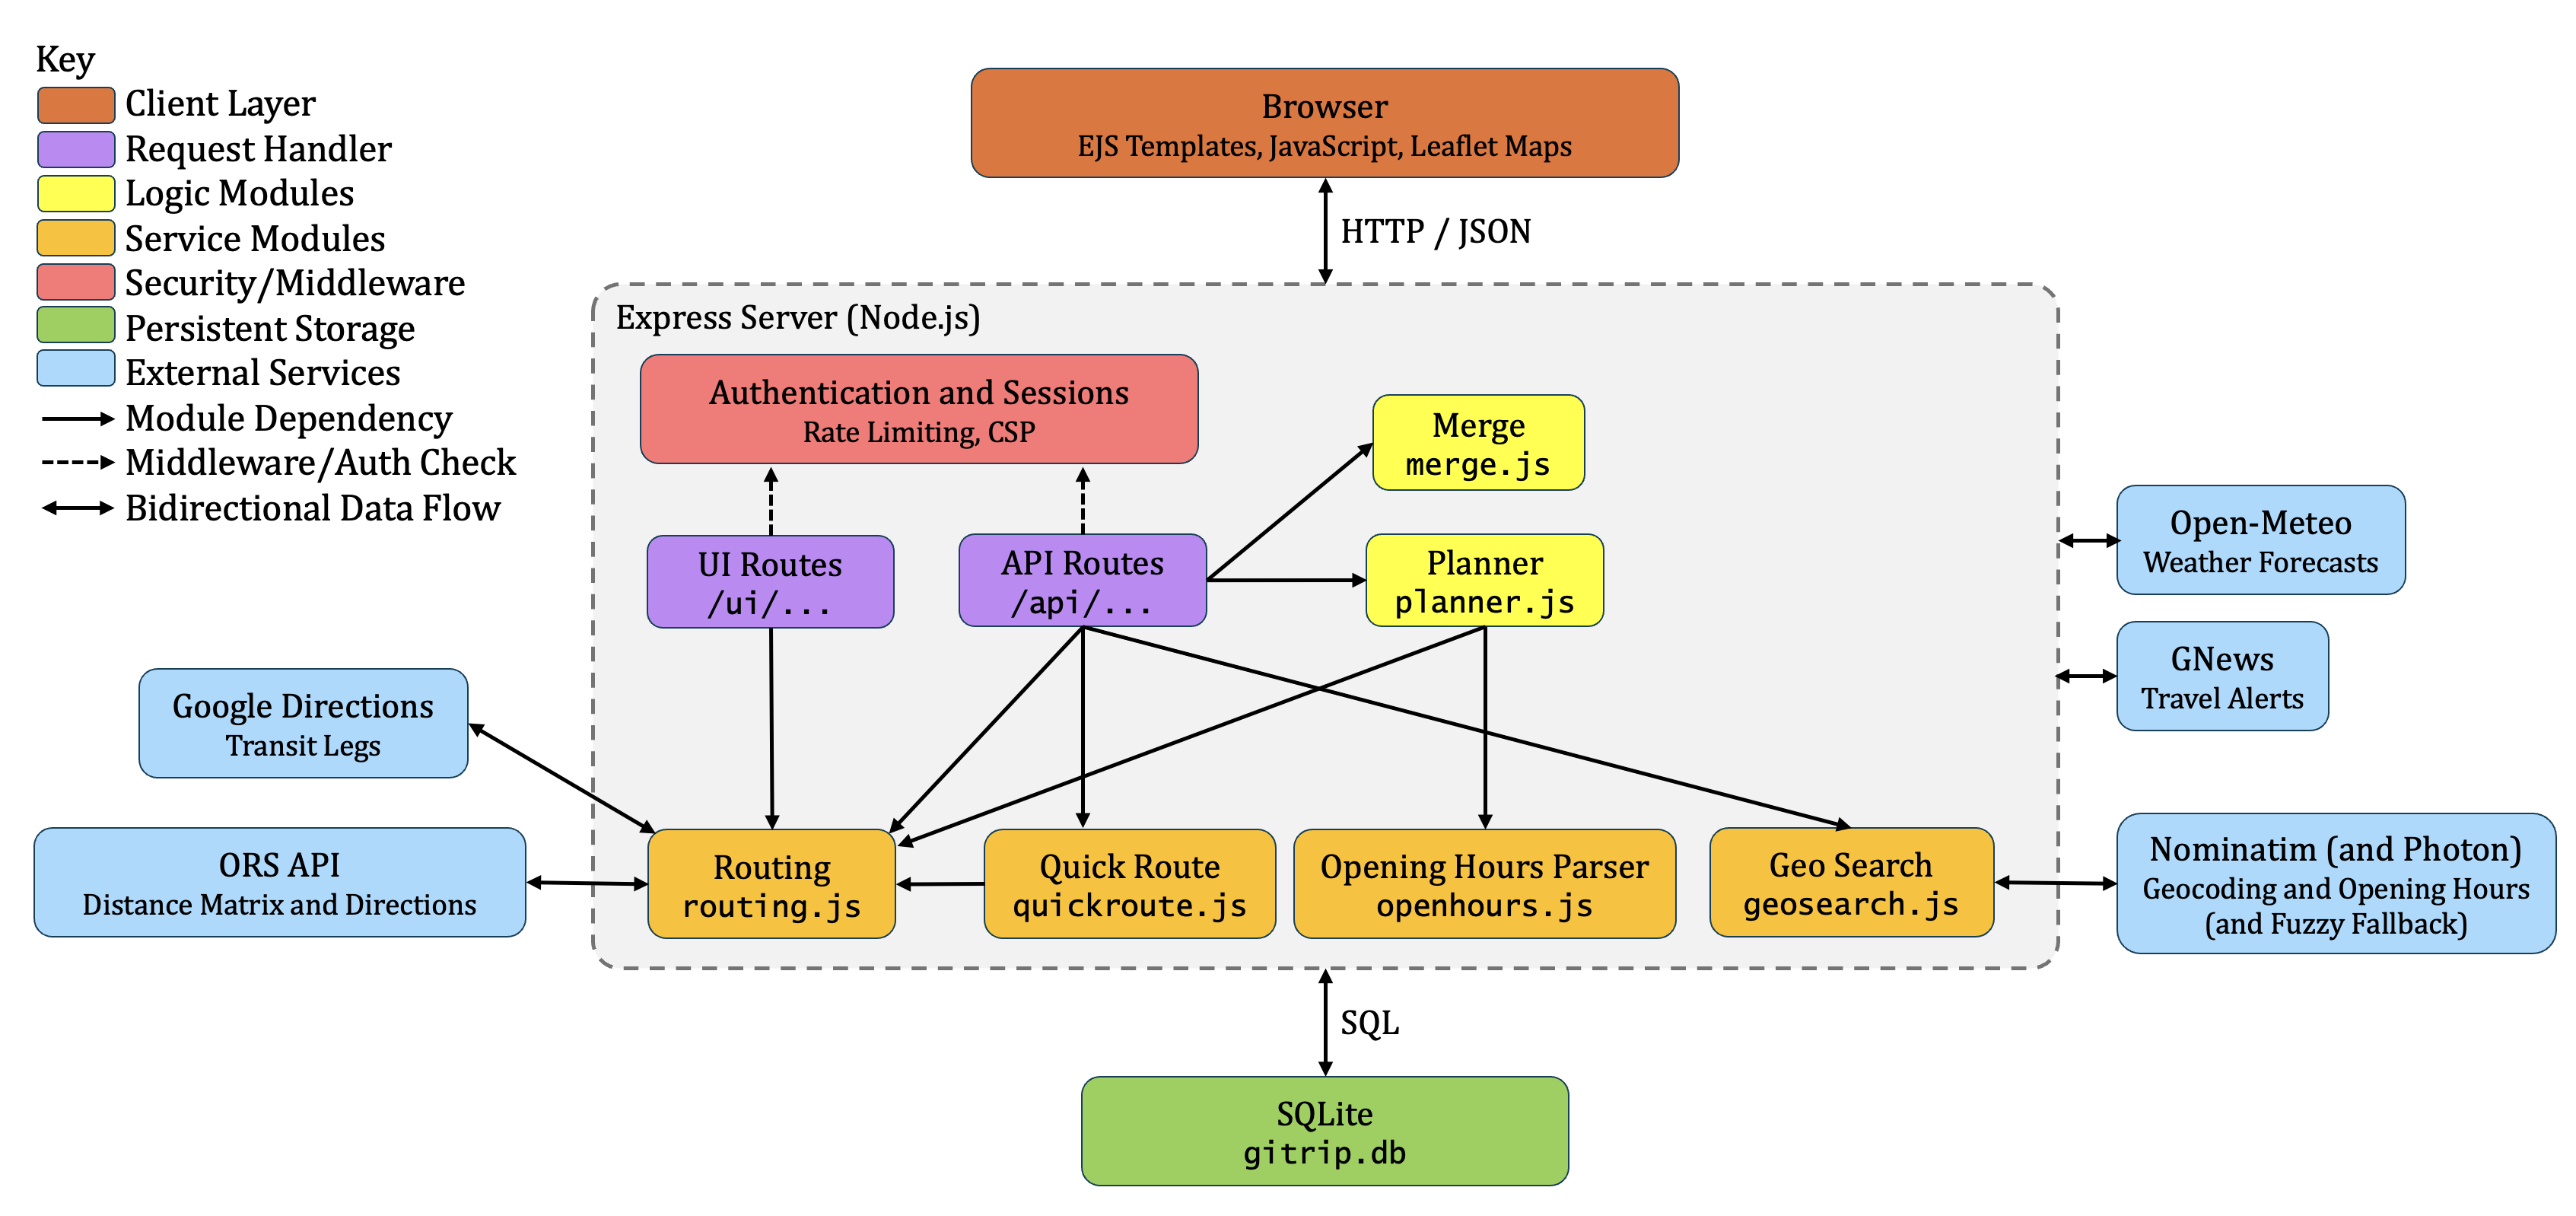
\includegraphics[width=\textwidth]{Chapter5/architecture-diagram.png}
  \caption{High-level system architecture of GiTrip.}
  \label{fig:architecture}
\end{figure}

\section{Data Model and Repository Semantics}
GiTrip's database schema includes the following core tables:
\begin{itemize}
  \item \textbf{repos:} repository metadata (title, owner, visibility, current
        branch, fork source), keyed by a Universally Unique Identifier (UUID).
  \item \textbf{branches:} named pointers to commits (head commit).
  \item \textbf{commits:} commit metadata and full snapshot storage.
        Each commit records its parent commit(s), forming a Directed Acyclic
        Graph (DAG) that represents the repository's version history.
\end{itemize}

Additional tables support authentication (\textbf{users}, \textbf{sessions}) and
social/collaboration (\textbf{repo\_collaborators}, \textbf{repo\_stars}).
Supporting planning features are stored in \textbf{travel\_alerts} and
\textbf{packing\_checklists}. Database indexes are defined on all foreign-key
columns (e.g., \texttt{commits.repo\_id}, \texttt{branches.repo\_id},
\texttt{repo\_stars.repo\_id}) to ensure query performance scales with data
growth.

Figure~\ref{fig:erd} shows the entity relationship (ER) diagram for GiTrip's data
model using Crow's foot notation. The core version-control triad (Repo, Branch, Commit) mirrors Git
semantics, while the embedded Snapshot structure captures itinerary-specific data
as JSON within each commit row. Solid-bordered entities are persisted as SQLite tables; dashed-bordered entities represent JSON structures embedded within the \texttt{snapshot} column of each Commit. Primary keys are underlined in the diagram. Crow's foot endpoints: double bar = exactly one, circle--bar = zero or one, fork--bar = one or many, fork--circle = zero or many.

\begin{figure}[H]
  \centering
  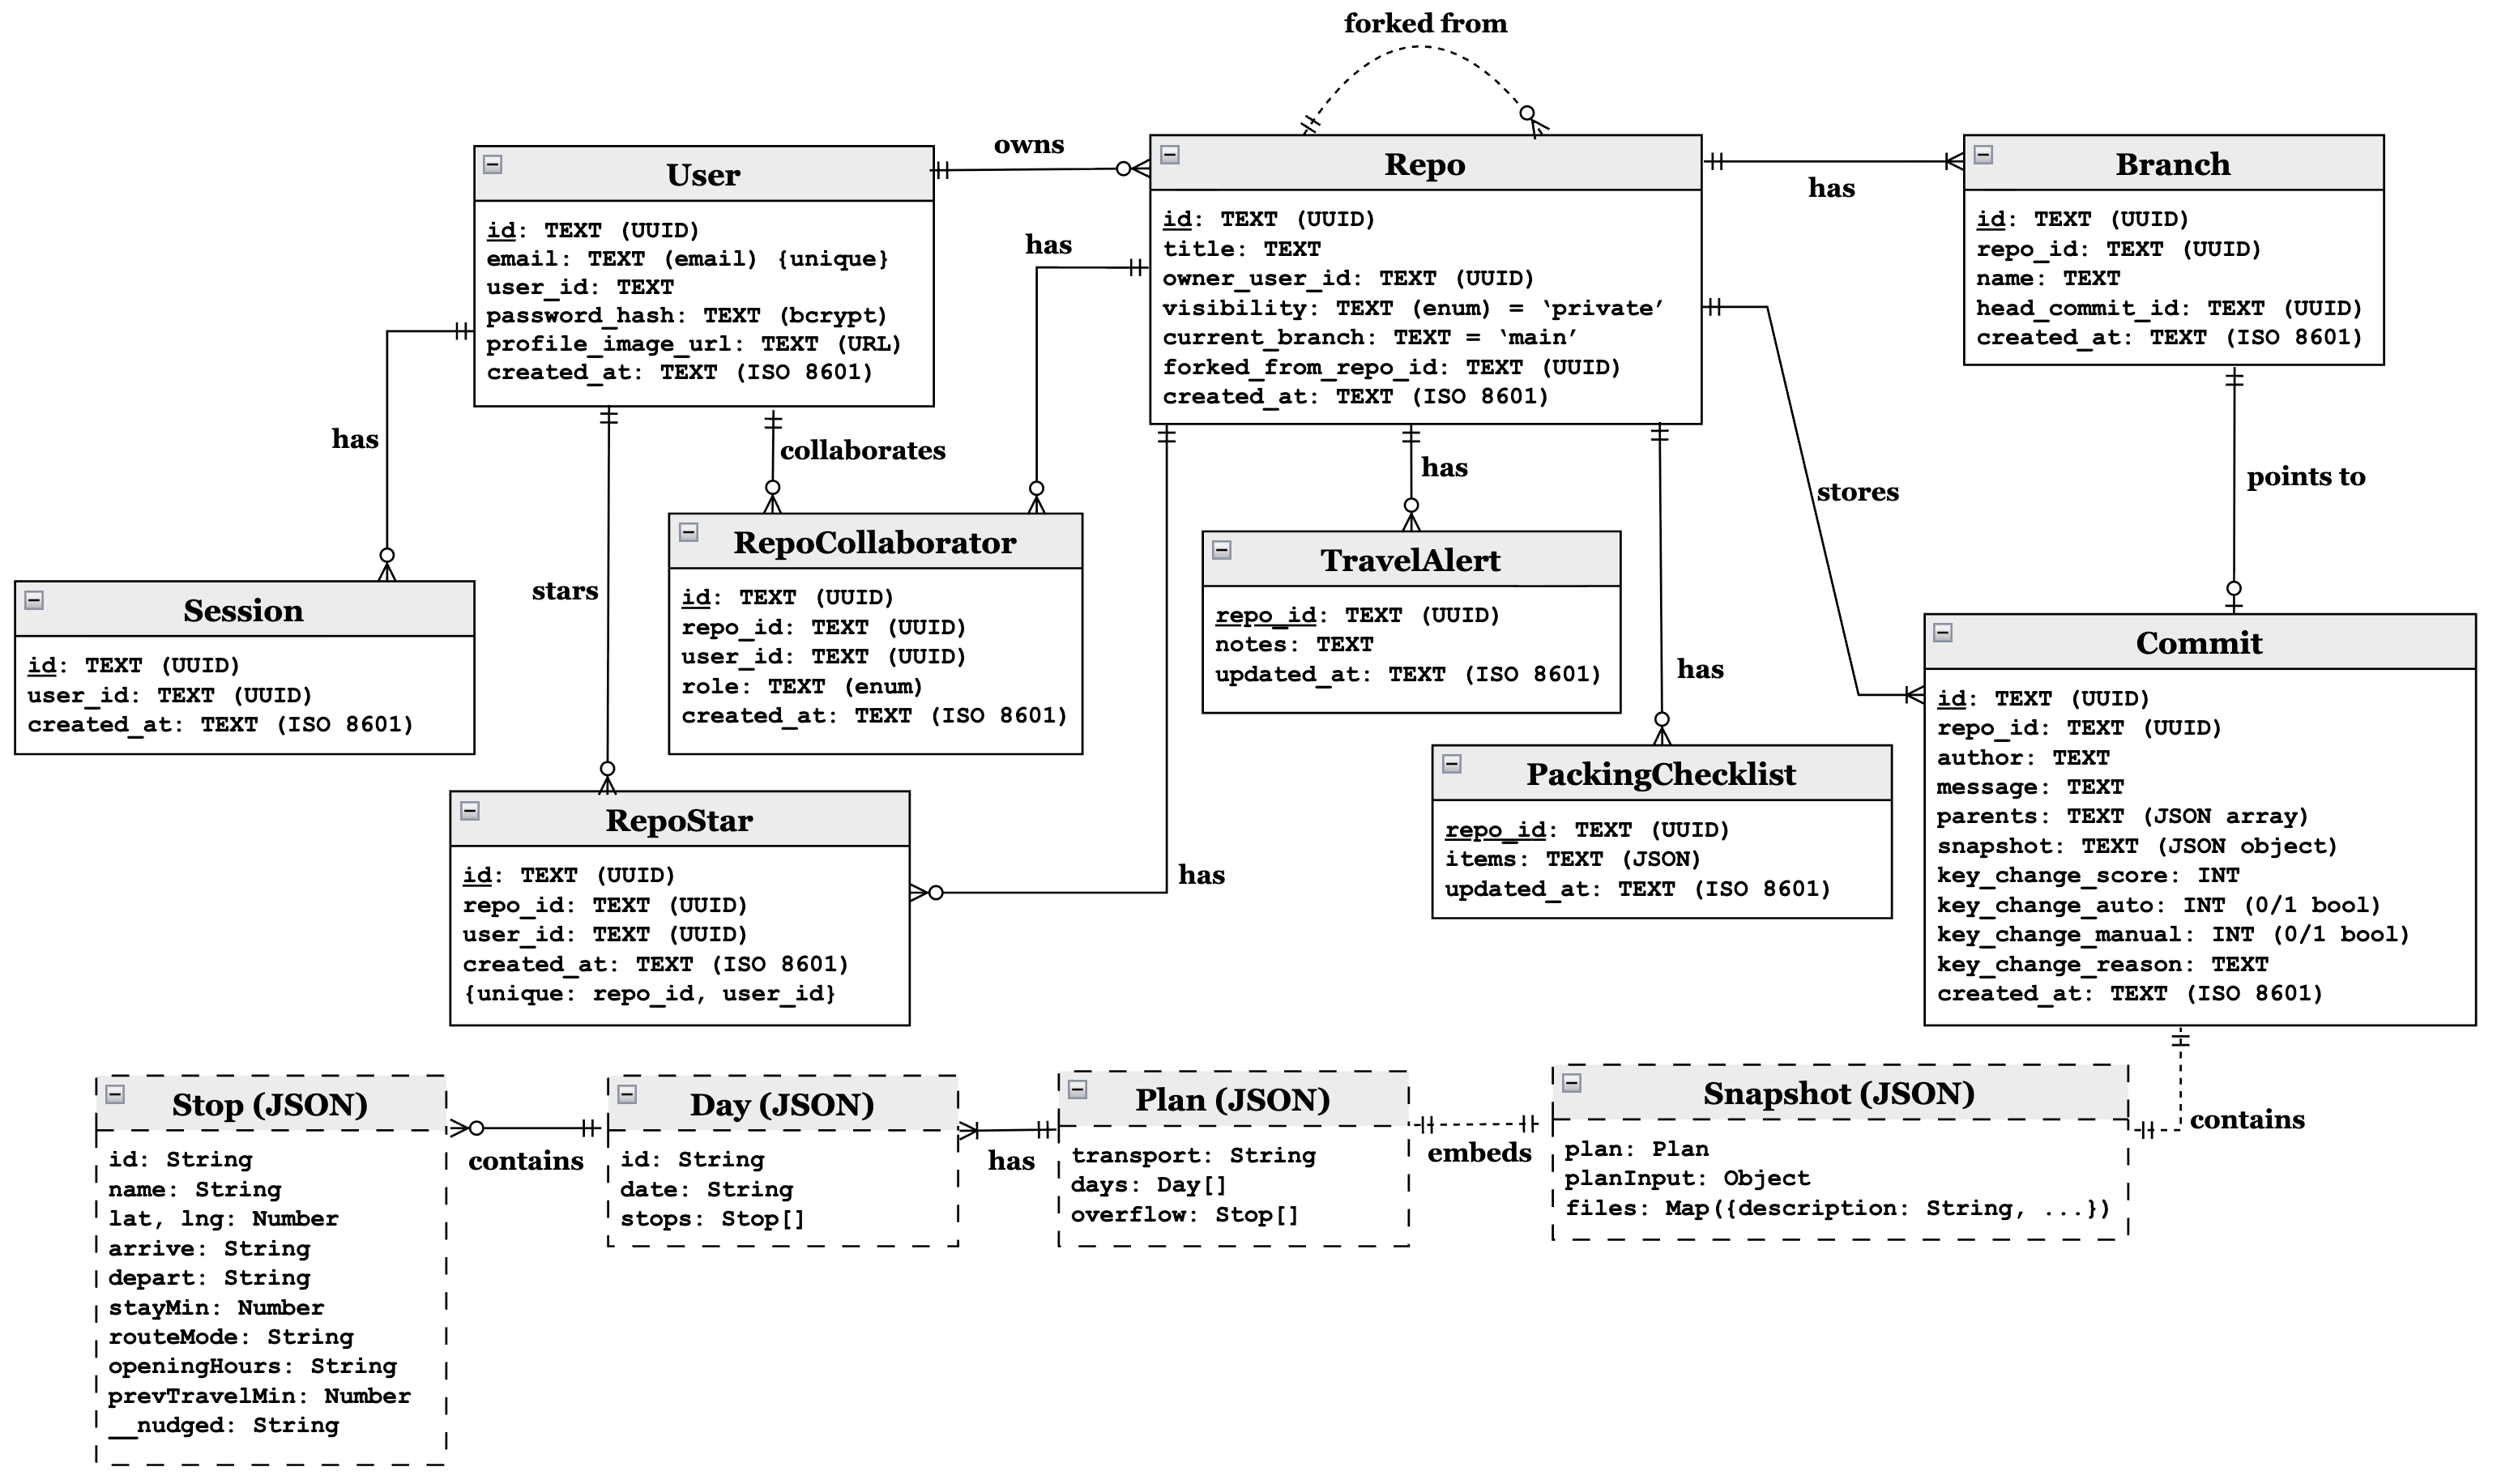
\includegraphics[width=\textwidth]{Chapter5/ER-diagram.png}
  \caption{Entity relationship diagram for GiTrip's data model.}
  \label{fig:erd}
\end{figure}

\subsection{Snapshot Storage}
Commits store complete plan snapshots. Snapshot versioning was selected over delta storage (method to store only the differences between versions) because it (i) simplifies branch switching and rollback (no delta replay), (ii) simplifies three-way merge (each tip contains a complete state), and (iii) remains feasible for the expected scale~\cite{ref_progit_snapshots}. Delta compression is noted as future work for production-scale repositories. Each snapshot contains:
\begin{itemize}
  \item \texttt{snapshot.plan}: the itinerary (days and stops).
  \item \texttt{snapshot.planInput}: planner inputs for reproducibility and UI defaults.
  \item \texttt{snapshot.files}: a key-value map for branch-level metadata. For example, the trip description (\texttt{files.description}), which collaborators can edit independently on separate branches. The merge engine performs per-key three-way merging on this map, detecting conflicts when both sides change the same key.
\end{itemize}

\subsection{Plan Schema}
A plan includes:
\begin{itemize}
  \item \texttt{transport} mode (driving/walking/cycling/transit),
  \item \texttt{days[]} each with \texttt{id}, \texttt{date}, and
        \texttt{stops[]},
  \item each stop includes identity, location, scheduling, and routing metadata.
\end{itemize}

Stops also carry planner constraint fields such as strict ordering, time windows,
fixed-time flags, and opening-hours strings. A \texttt{\_\_nudged} marker records
explainable adjustments made by the scheduler (e.g., nudged due to opening
hours).

\subsection{Module Structure}
Figure~\ref{fig:uml_class} shows the Unified Modeling Language (UML) class diagram for GiTrip's server-side
modules. Each module is represented as a class with its exported functions as
public operations (\texttt{+}) and internal helper functions as private
operations (\texttt{-}). The \texttt{Server} module acts as the central
orchestrator, delegating to specialised modules for planning, merging, routing,
and geocoding. \texttt{TTLCache} is the only formal JavaScript class in the
codebase; all other modules use the CommonJS \texttt{module.exports} pattern. In the diagram, dashed open arrows denote $\langle\!\langle$use$\rangle\!\rangle$ dependencies and the filled diamond denotes composition (Server owns TTLCache instances).

\begin{figure}[H]
  \centering
  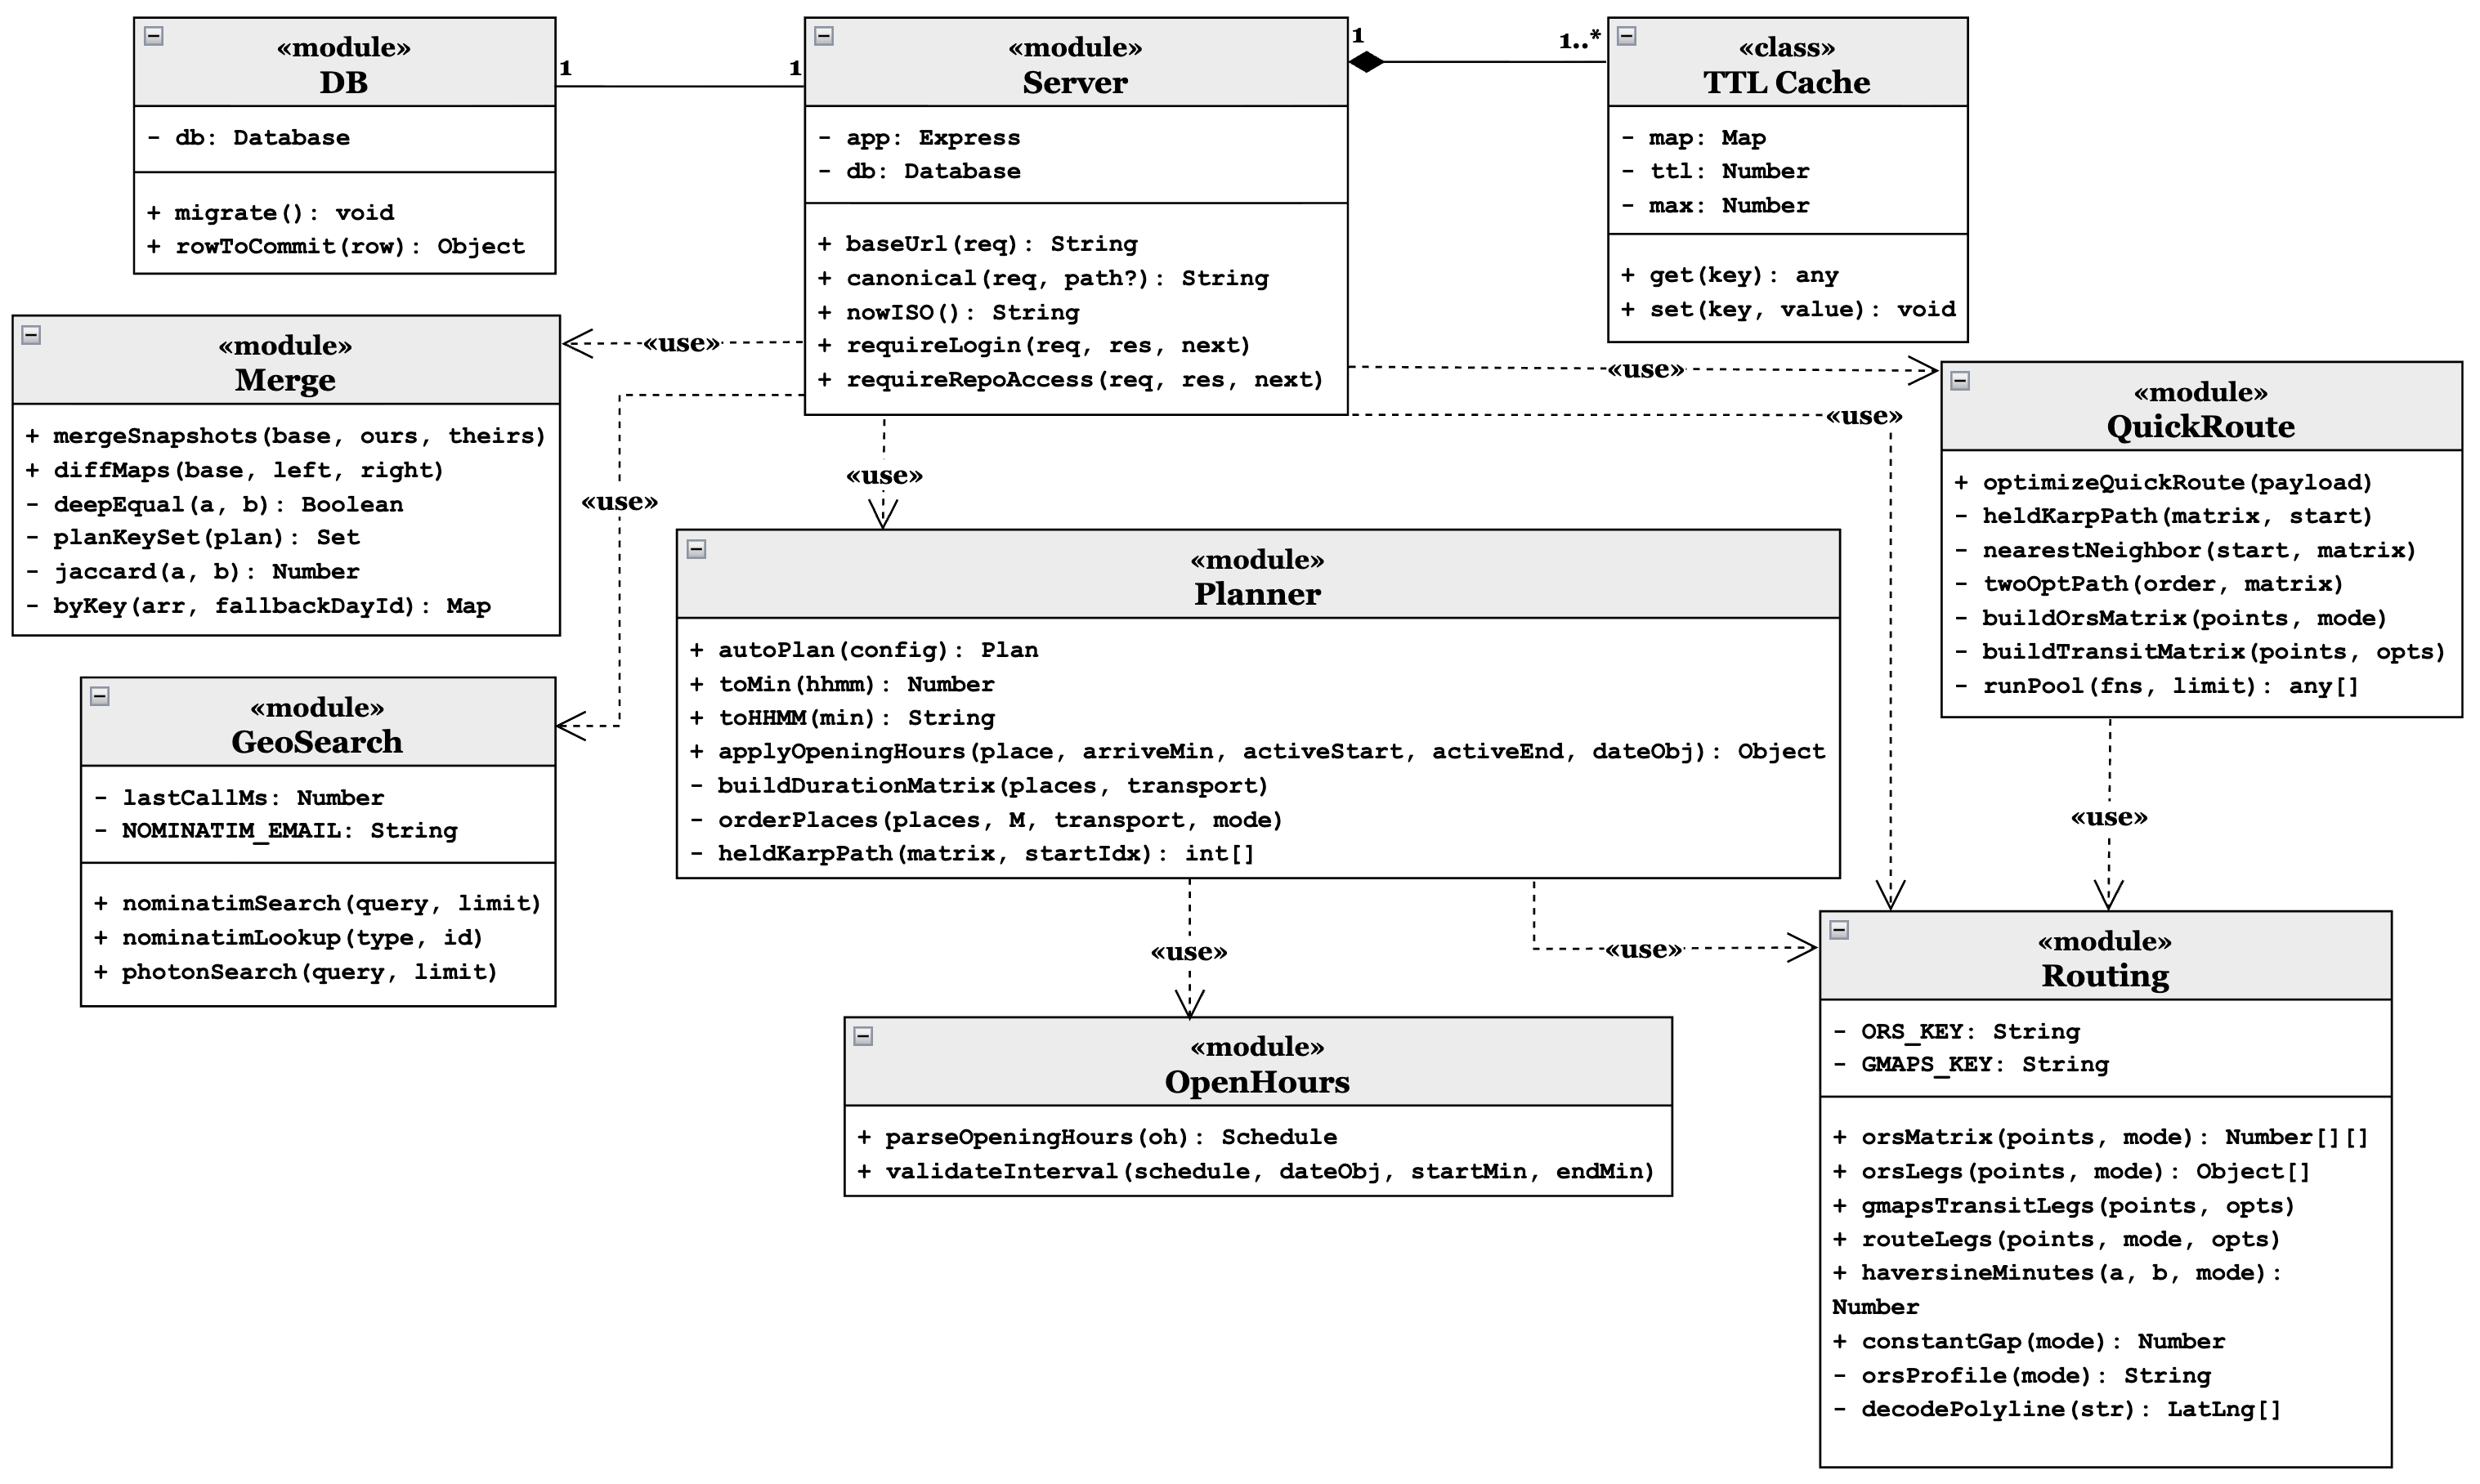
\includegraphics[width=\textwidth]{Chapter5/uml-class-diagram.png}
  \caption{UML class diagram for GiTrip's server-side modules.}
  \label{fig:uml_class}
\end{figure}

\section{Routing and Geocoding Design}
\subsection{Place Search}
GiTrip proxies Nominatim~\cite{ref_nominatim} search/lookup via server endpoints to enable caching and rate limiting. Results are re-ranked using approximate string matching to prioritise substring matches and reduce diacritic/punctuation sensitivity \cite{ref_navaro_string_matching}. Since Nominatim performs exact matching against its index, near-miss queries (e.g.\ ``stick n sushi'' for ``Sticks'n'Sushi'') can return zero results. To address this, GiTrip falls back to Photon~\cite{ref_photon} when Nominatim returns no matches. Photon is an open-source geocoder built on Elasticsearch that indexes the same OpenStreetMap data with n-gram tokenisation and typo tolerance, providing fuzzy search without requiring a separate dataset. The fallback is transparent: Photon results are returned in the same shape, with \texttt{opening\_hours} set to null since Photon does not expose that field.

\subsection{Routing Providers and Fallback}
Routing serves two purposes. First, ORS matrix endpoints compute pairwise travel durations for route ordering (driving/cycling/walking). The matrix endpoint reduces API calls from $O(n^2)$ pairwise requests to a single request per optimisation run. Second, per-leg routing provides geometries for map visualisation; Google Directions is used for transit legs, including decoding polylines and extracting step-level sub-modes to distinguish walking approach segments.

For non-transit modes, GiTrip requests a travel-time matrix from OpenRouteService~\cite{ref_ors_matrix}. For transit, GiTrip uses Google Directions API~\cite{ref_google_directions_api} for
sequential legs. When providers fail or are
unavailable, GiTrip falls back to Haversine-based time estimates (computing approximate travel duration from straight-line distance with mode-dependent speed assumptions) for ordering, and constant default travel gaps per mode (e.g., 15 minutes for driving, 30 minutes for transit) as a safety margin when no routing data is available at all. This design ensures the planner remains usable even in degraded conditions, which is important for evaluation environments and offline/limited-connectivity contexts.

\section{Auto-scheduler Design}
The scheduler must construct a feasible plan that respects constraints. GiTrip's
scheduler is designed around four stages:
\begin{enumerate}
  \item \textbf{Matrix construction:} request pairwise travel durations (when
        available).
  \item \textbf{Ordering:} determine visit order using strict order constraints
        when provided; otherwise use Held-Karp exact solver for small instances
        ($N \leq 12$) \cite{ref_tsp_study} or Nearest Neighbour with 2-Opt
        refinement for larger instances
        \cite{ref_nn_tsp,ref_nn_2opt_hybrid}.
  \item \textbf{Packing into days:} greedily place stops into day windows while
        maintaining non-overlap and travel gaps.
  \item \textbf{Constraint enforcement:} apply opening hours, desired windows,
        and fixed-time constraints; if a stop cannot fit, spill it to a
        subsequent day or overflow.
\end{enumerate}

Given ordered stops $S_1,\dots,S_n$, per-leg travel $T_i$ (minutes from $S_{i-1}$ to $S_i$), stay durations $D_i$, active window $[A,B]$, break $b$, and focus offset $f$:
\[
a_1 = A+f,\quad d_1=a_1+D_1,\quad
a_i = d_{i-1}+b+T_i,\quad d_i=a_i+D_i \ (i>1).
\]
If $(a_i,d_i)$ violates a desired window or opening-hours constraint, the scheduler shifts to the nearest valid interval inside $[A,B]$; otherwise, it spills to the next day's $A+f$. The user preference (compact vs.\ sparse) controls additional free time after each stop.

\subsection{Opening Hours Nudging}
Opening hours are treated as a hard-ish constraint: if the proposed interval
falls in a closed period, the scheduler nudges to the next open slot where
feasible; otherwise the stop is rejected for that day. This is crucial for
feasibility and directly addresses common itinerary failures in real planning.

\subsection{Compact vs Sparse Modes}
To improve user control over schedule density, the scheduler supports
``compact'' and ``sparse'' modes. Compact mode packs stops tightly, while sparse
mode distributes stops across the active window by inserting additional gap time.
This preference improves perceived usefulness because different trip styles (e.g.,
city sprint vs relaxed exploration) require different pacing.

\subsection{Design Trade-offs and Pseudocode}
A key design trade-off in the scheduler is the choice of NN ordering over more sophisticated approaches such as exact TSP solvers~\cite{ref_tsp_study} or meta-heuristics~\cite{ref_tsp_local_search}. NN was selected because: (i) it runs in $O(n^2)$ time and performs acceptably for typical trip sizes ($n \le 50$ stops), (ii) it avoids the implementation complexity and computational cost of exact solvers, and (iii) API quota constraints make it infeasible to request large distance matrices repeatedly during interactive editing. For trips with more than 50 stops, the scheduler divides the itinerary into day-sized chunks and optimises each independently, which maintains reasonable performance while accepting some suboptimality in cross-day transitions. The full pseudocode for the auto-scheduler is presented in Chapter~\ref{ch:implementation} (Algorithm~\ref{alg:planner}).

\section{Merge Design}
GiTrip implements a Git-style three-way merge for snapshots. The merge process
uses:
\begin{itemize}
  \item a \textbf{base} snapshot, the lowest common ancestor (LCA),
  \item \textbf{ours} and \textbf{theirs} snapshots (branch heads),
  \item a merge engine producing a merged snapshot plus a list of conflicts.
\end{itemize}

The fundamental principle, inherited from Git's merge model, is that a conflict
only arises when \textbf{both} branches express a different opinion about the
same data relative to the base. If only one branch changes a stop (or deletes
it) and the other leaves it untouched, the merge engine cleanly accepts the
change---just as \texttt{git merge} auto-resolves one-sided edits. For example,
if one branch deletes a stop and the other never touched it, the deletion is
accepted; a conflict is raised only if the other branch also \textit{edited}
that stop, creating a genuine disagreement.

Figure~\ref{fig:merge_flow} illustrates the full decision logic of the merge
engine. The engine first iterates all file keys, recording conflicts or taking the changed side, then checks plan divergence. If both sides changed the plan identically, either is taken. If both changed the plan structure and their stop-key Jaccard similarity is below~0.4, a whole-plan conflict is raised. Otherwise, per-stop merging chains through deletion, time, and field checks. The result is stabilised by deterministic ordering before output.

\begin{figure}[H]
  \centering
  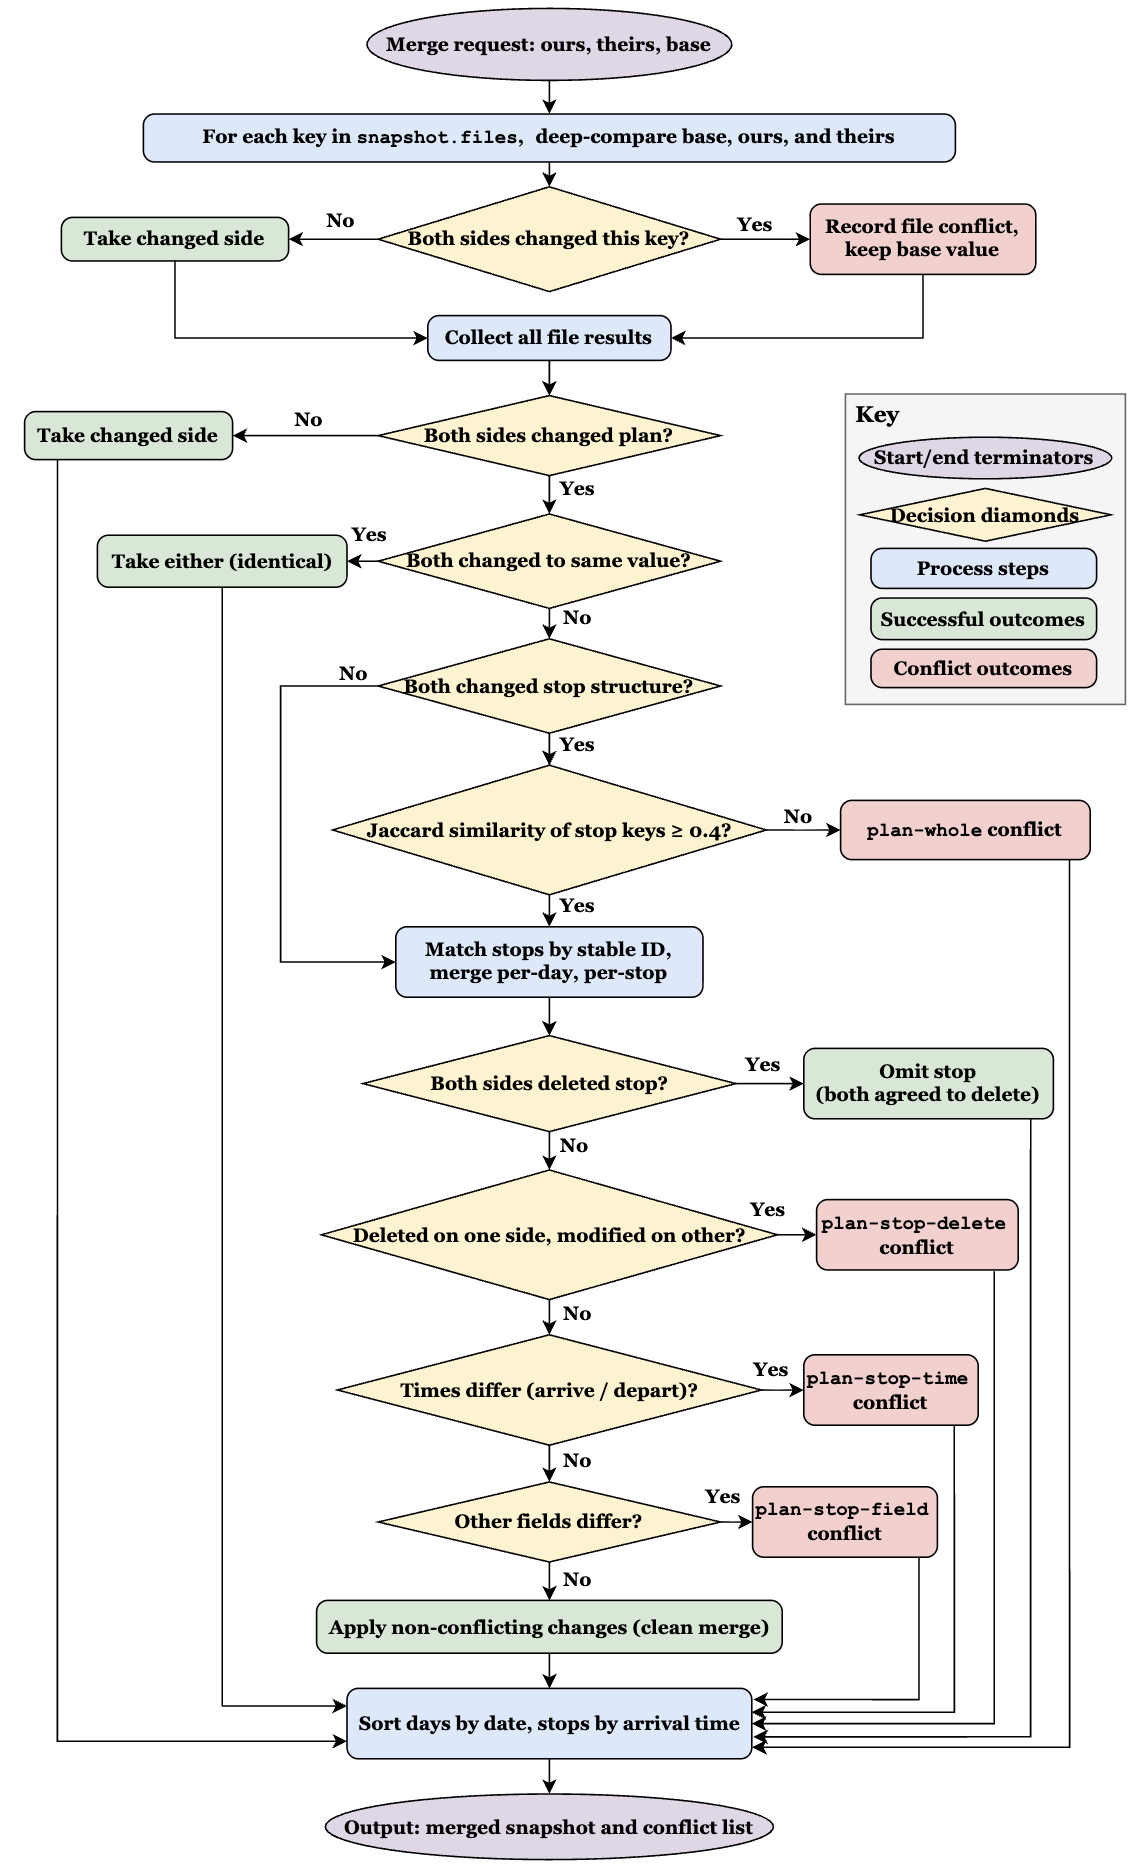
\includegraphics[width=0.9\textwidth]{Chapter5/merge-flowchart.png}
  \caption{Three-way merge decision flowchart.}
  \label{fig:merge_flow}
\end{figure}

\subsection{Equality and Stability}
Early merge implementations that relied on \texttt{JSON.stringify} can be brittle
because key insertion order may differ and \texttt{undefined} values are dropped.
The final implementation uses deep structural equality, making comparisons
key-order independent.

Additionally, merged ordering is stabilised by sorting days by ISO date and
sorting stops by arrival time (then name). This reduces surprising reordering
after merges.

\subsection{Conflict Types}
Conflicts surfaced include:
\begin{itemize}
  \item \textbf{file:} both sides changed the same key in \texttt{snapshot.files} (e.g., the trip description).
  \item \textbf{plan-stop-time:} both sides changed arrival/departure times
        differently for the same stop.
  \item \textbf{plan-stop-delete:} one side deleted a stop while the other
        modified it.
  \item \textbf{plan-stop-field:} times agree but both sides changed selected
        fields differently (e.g., name, lat/lng, notes, stayMin, routeMode).
  \item \textbf{plan-whole:} plans diverged heavily (Jaccard similarity of
        stop-key sets below 0.4), requiring whole-plan selection.
\end{itemize}

This set is intentionally constrained to keep the UI manageable for non-experts
while still preventing silent data loss.

\section{User Interface Design}
GiTrip uses server-rendered pages enhanced by client-side JavaScript. Two
interactive surfaces support editing:
\begin{itemize}
  \item \textbf{Timeline editor:} draggable blocks and handles adjust
        arrival/departure times with snapping and constraint clamping.
  \item \textbf{Map editor:} draggable numbered markers adjust stop coordinates
        and update route geometry.
\end{itemize}

\subsection{Easy Mode vs Git Mode}
In Q8 of the survey, asking if there are any concerns with this project, 6/11 respondents mentioned that \textit{Git} concept may be complicated for users without a technical background. To reduce this cognitive overhead while preserving versioning power for advanced users, the ``Git mode'' toggle button was invented. When turned off, the UI replaces \textit{Git}-related terminologies with task-oriented wording (e.g., ``Save trip'' rather than ``Commit''), while keeping the functionality same. In addition, when turned off, the advanced auto-scheduler workflow is complemented by an easy-mode scheduling path (Appendix~\ref{appx:diagrams}), where users can create a trip by entering a bullet-point stop list and letting the system generate and commit a feasible itinerary. This design keeps the novice workflow ``single-track'' (plan $\rightarrow$ save $\rightarrow$ refine) while allowing expert users to opt into full version-control semantics without losing compatibility with the stored data.

GiTrip therefore includes a mode toggle:
\begin{itemize}
  \item \textbf{Easy mode:} hides branches/commits/merge; offers ``Save trip''
        with non-fast-forward friendly behaviour.
  \item \textbf{Git mode:} exposes full repository semantics and merge UI.
\end{itemize}

This design supports two user personas without splitting the product into
separate applications.

\subsection{Quick Explore Mode}
The ``Quick route'' page adopts a \textit{Google Maps}-like interaction style to minimise onboarding friction: the primary surface is a map plus a simple stop list, and the user can immediately compute an optimised order and per-leg travel times without first understanding repositories, branches, or commits. This design matches a common mental model for trip planning (enter places $\rightarrow$ see route $\rightarrow$ iterate), and it also includes a bookmark feature that lets users save places and immediately compute the entire route when pressed. Crucially, \textit{GiTrip} connects this streamlined workflow back to the full versioned system via ``Save as Repository'': once the user is satisfied with a route, the system creates a repository and an initial snapshot commit containing the generated plan. This provides a low-friction entry point for new users, while still enabling the richer repository workflow (timeline editing, map refinement, branching, and merging) when needed.

\section{Security, Privacy, and Accessibility Design}
GiTrip includes several practical web security measures:
\begin{itemize}
  \item session cookies are HttpOnly and SameSite=Lax,
  \item security headers include CSP, frame blocking, and HTTP Strict Transport Security (HSTS) in production,
  \item rate limiting is applied globally and more strictly on sensitive
        endpoints (four tiers: global, API, geo search, and authentication),
  \item prepared statements are used for SQLite queries to reduce SQL injection
        risk,
  \item error responses return generic messages to users while logging full
        details server-side, preventing information leakage of internal paths
        or stack traces.
\end{itemize}

Accessibility is guided by WCAG 2.2~\cite{ref_wcag22}. The UI uses labelled
controls and avoids information conveyed only by colour; however, interactive
map/timeline controls remain a known accessibility challenge and are discussed as
a limitation.
